
\documentclass[11pt]{article}

%\usepackage[top = 1 inch , bottom = 1 inch , left =0.5 inch , right =0.5 inch]{geometry}
\usepackage{amsmath}
\usepackage{amssymb}
\usepackage[top =1 in  , bottom =1 in , left=0.5 in , right = 0.5 in]{geometry}
\usepackage{graphicx}
\newcommand{\BibTeX}{{\sc Bib}\TeX}
\usepackage{url}
\begin{document} %documents starts here


%title

\title {Physics Behind the simulation : A CS296 Report by Group 13 }
\author {\emph{Group 13} \\ %Group members 
	\emph{Pintu Lal Meena} \\
	 \textrm{120050018} ,  \textsf{pintulalmeena@hotmail.com} \\
	\emph{Pranay Dhondi } \\
	\textrm{120050054} , \textsf{pranaydhondi@gmail.com} \\
	\emph{Shivam Garg}\\
	\textrm{12D020036} , \textsf{shivam.garg55@gmail.com}}
\date{\today}   % this will represent the current date
\maketitle
%\begin{abstract}
%This Document is about extra elements added in box2d and their  physical behaviour and properties .
%\end{abstract}
\section{Introduction}
This report explains the physical behaviour and properties of extra
added elements in box2d . This is a part of assignment given in lab 03 of CS 296.
\newline
Following elements are added by us :
\begin{itemize}
\item Wall 
\item Ball
\item Wedge
\end{itemize}
\section{Physics behind the simulation}

\subsection{Wall}
Assumed that the wall is fixed  and takes an elastic collision \cite{ref1} (i.e., Coefficient of restitution \cite{ref2} is 1)
\newline
\begin{center}
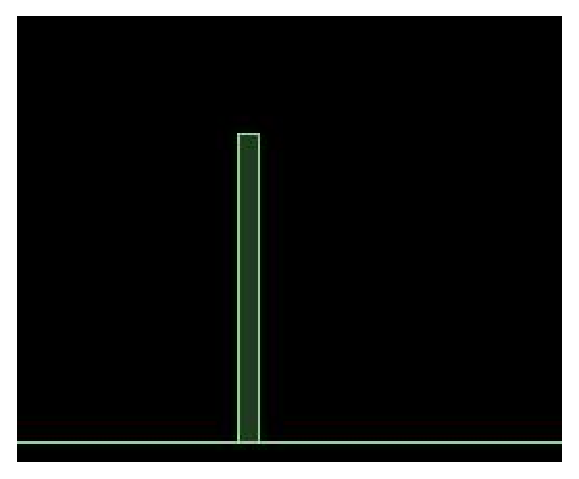
\includegraphics[scale=0.9]{wall}
\end{center}
%\paragraph{Equations}
 When there is collision between wall and ball , there is a perfect elastic collision . Momentum of these objects is not conserved because force is acting on wall to keep it fixed \cite{ref1}. This is governed by the following equations:
%\subparagraph{Assumpitons}
% assume that the mass of ball is m(in kg) and mass of wall is M(in kg) . u,U be the intial velocities of ball and wall (in meter/second) respectively.
% v,V be the final velocities of ball and wall(in meter/second) respectively . we have U=V=0 because wall is fixed . cofficient of restitution at wall =1.
\begin{eqnarray}
e & = &\frac{V-v}{u-U}  \\
1 & = &\frac{V-v}{u-U} \nonumber  \label{eq:simp1} \\
u - U & = & V-v \nonumber  \label{eq:simp1} \\
 v & = & -u  \label{eq:simp1} 
\end{eqnarray}
\\
\\
$m$: Mass of ball ($kg$) \\
$M$: Mass of wall ($kg$) \\
$u$: Initial velocity of ball ($m/s$) \\ 
$U$: Initial velocity of wall ($m/s$) \\
$v$: Final velocity of ball ($m/s$) \\  
$V$: Final velocity of wall ($m/s$) \\
$e$: Coefficient of restitution \\ 
 %\[\frac{V-v}{u-U) \]
 %\begin{displaymath}
 %e=1=\frac{V-v}{u-U)
 % V=U =0 .
% % v=-u.
 %\end{displaymath}
 
\subsection{Ball}
Let us assume that the mass of the ball which was already present be  $m (kg)$ . The mass of the new ball added is the same as  mass of the ball already present , i.e, $m (kg)$ . Ball is smooth.
\newline
\begin{center}
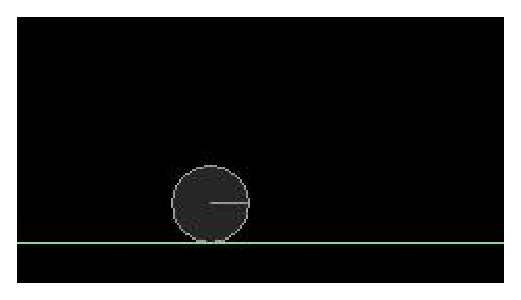
\includegraphics{Ball}
\end{center}
%\paragraph{Equations} When the ball hits the wall then its equation is same as equation (1) .
%\newline
When the ball which was actually present hits the new ball , since we have assumed that the collison is elastic and no external forces are acting on the system (two balls)  momentum is conserved. This is governed by the following equations: \\
%\subparagraph{Assumptions} Let the mass of the two balls be m (in kg) ,
%u1=0 , u2 be the initial velocities of ball at rest (B1) and incoming ball (B2) respecively . v1 , v2 be the final velocities of balls  B1 and B2 respecively.

\begin {eqnarray}
  mu_1 + mu_2 & = & mv_1 + mv_2 \\
  u_2 & = & v_1 + v_2 \label: (eq:simp3)  \\
  from & equation 1 & \nonumber \\
  1 & = &  \frac{v_2-v_1}{u_1-u_2} \nonumber \\
  -u_2 & = & v_2 - V_1 \\
  from & equation 4 , 5 & \nonumber \\
  v_1 & = & u_2 \nonumber \\
  v_2 & = & 0  \nonumber 
\end{eqnarray}
\\
\\
$m$: Mass of both the ball ($kg$) \\
$u_1$: Initial velocity of the ball at rest ($B_1$) ($m/s$) \\ 
$u_2$: Initial velocity of the incoming ball ($B_2$) ($m/s$) \\
$v_1$: Final velocity of $B_1$ ($m/s$) \\  
$v_2$: Final velocity of $B_2$ ($m/s$) \\
\subsection{Wedge\cite{ref3}}
Wedge is smooth and friction less.
\newline 
\begin{center}
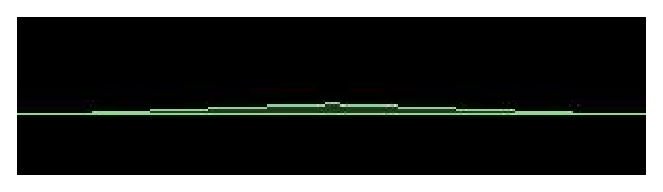
\includegraphics{wedge}
\end{center}
%\paragraph{Equations} 
%Assume that wedge be fixed and angle of inclination be theta . Acceleration due to gravity is g (m/s 2).
When the ball moves on the wedge the normal reaction (in Newtons) will be \[ mg\cos(\theta)\] 
The ball experiences  retardation (in Newtons) due to force\[ mg\sin(\theta)\] if ball goes up the wedge and  accelaration  by the same amount of force  if the ball moves down the wedge .
\begin{eqnarray}
Normal Reaction by wedge & = & mg\cos\theta \\
Accerlation Retardation experienced by body & =  & g\sin\theta
\end{eqnarray}
\\
\\
$m$: Mass of both the ball ($kg$) \\
$g$: Acceleration due to gravity ($kgm/s^2$) \\
$\theta$: Angle between the ground and slope ($radian$)\\
\section{Conclusions}
The 3 new elements added to the Box2d simulation display laws of conservation of momentum, concept of restitution, normal and tangential forces.  
%   Above report has images of files added in box2D , equations that they follow at collisions and their physical properites .
%\begin{thebibliography}{9} 
% to start a new reference.
 %%\emph{\LaTeX: A Document Preparation System}. Addison Wesley, Massachusetts, 2nd Edition, 1994. 
  %\end{thebibliography} 
\bibliographystyle{plain}
\bibliography{cs296_report_13}
\end{document}
